\documentclass[hyperref]{beamer}
\usepackage{lmodern}
\usepackage{graphicx}
\usepackage{caption} % Coloured captions

% 使用Ilmenua主题
\usetheme{Ilmenau}
\usepackage{xeCJK}
% 设置英文默认字体
\setmainfont{Ubuntu}
% 设置中文默认字体
\setCJKmainfont{Noto Serif CJK SC}

\title{Tune Performance \\ Domain Specific Language-Halide}
\author{wegatron} 
\date{\today} 
\begin{document}
%\logo{\includegraphics[scale=0.14]{logo-SF}}
\begin{frame}
\titlepage
\end{frame} 

\begin{frame}
\frametitle{Table of contents}
\tableofcontents
\end{frame} 


\section{性能相关的那些事}
\begin{frame}
\frametitle{性能挑战}
\begin{figure}[H]
  \centering
  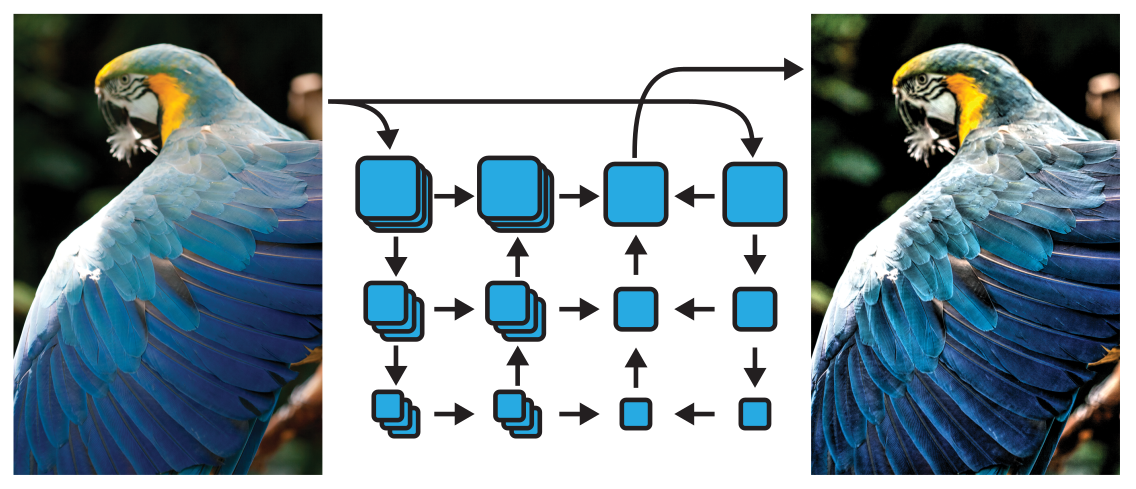
\includegraphics[width=10cm]{laplacian_filter.png}
  \caption{在实际应用中, 我们往往需要绞尽脑汁对算法做各种优化, 以满足在移动设备上的流畅运行.}
  \label{fig:laplacian-filter}
\end{figure}
\end{frame}

\begin{frame}
  \frametitle{实例分析-初始代码}
  \begin{figure}[H]
    \centering
    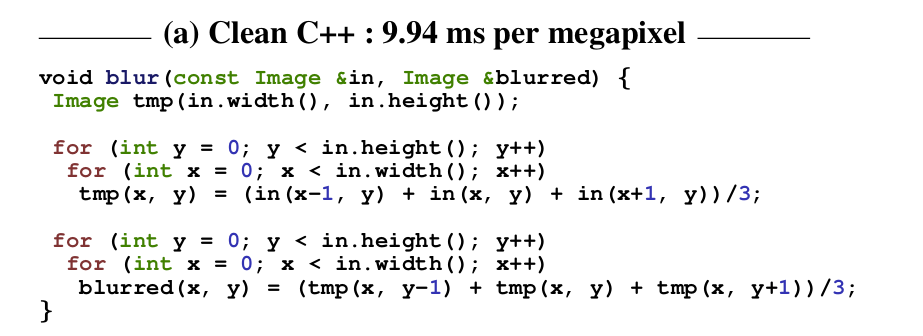
\includegraphics[width=10cm]{clean_c++.png}
    \caption{box filter simple c++ code}
    \label{fig:box-simple-c++}
  \end{figure}
\end{frame}

\begin{frame}
  \frametitle{实例分析-优化后的代码}
  \begin{figure}[H]
    \centering
    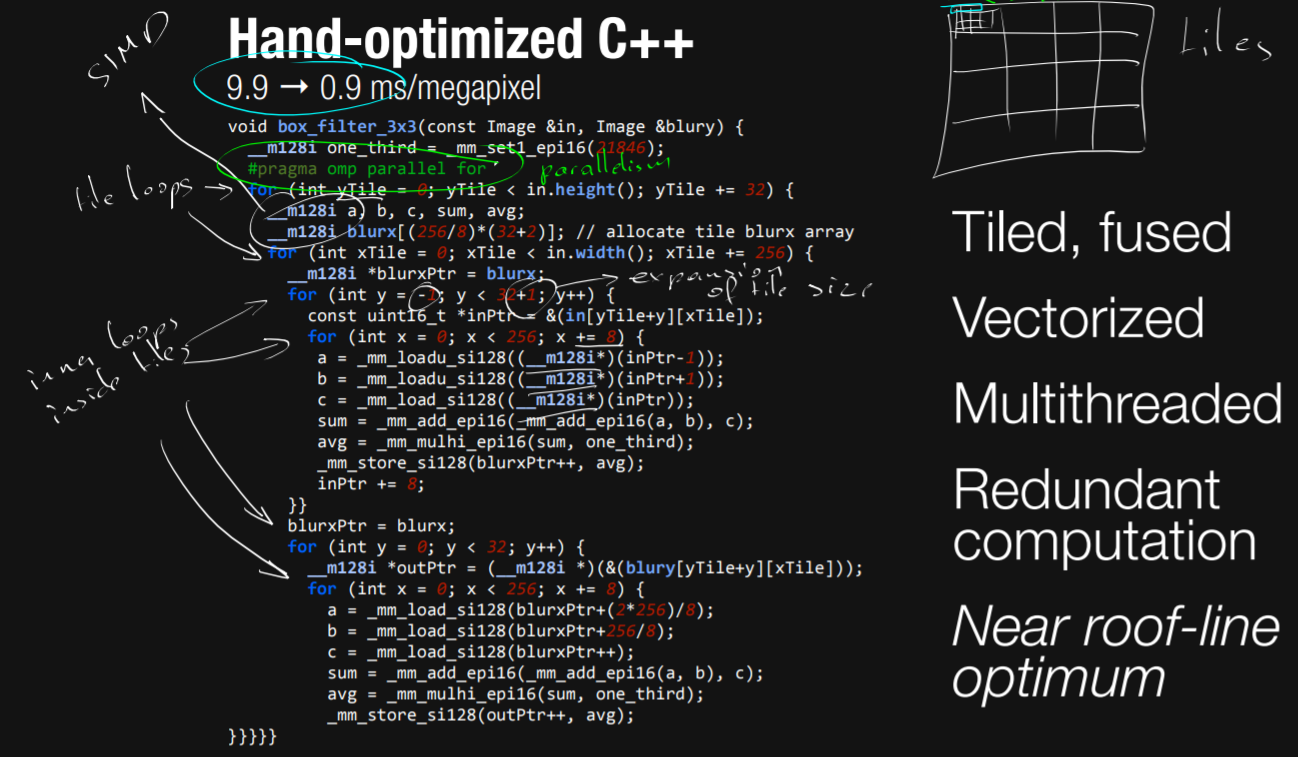
\includegraphics[width=10cm]{fast_c++.png}
    \caption{\tiny 使用矢量计算, tiling, 并行优化之后的快10倍的代码}
    \label{fig:box-fast-c++}
  \end{figure}
\end{frame}

\begin{frame}
  \frametitle{影响因素分析}
  以出行做类比:
  \begin{itemize}
  \item 算法的设计/参数——计算量(O(n), O($n^2$), ...). \\出行的目的地/路线(抄小道)
  \item 代码实现. 重复计算/无效计算, 并行, 矢量计算, 内存操作. \\出行具体时间的安排(堵车, 等车...)
  \item 硬件能力. \\出行交通工具(步行, 骑车, 汽车, 飞机)
  \end{itemize}
\end{frame}

\section{性能优化的思考}
\begin{frame}
  \frametitle{优化方向}
  我们分两方向进行思考:
  \begin{itemize}
    \item Algorithm: 如何设计高效的算法(算法定义了计算量)
    \item Schedule: 如何将算法编码为高效的机器二进制码
  \end{itemize}
\end{frame}

\begin{frame}
  \frametitle{The Schedule}
  Schedule包含的内容:
  \begin{itemize}
  \item 遍历的顺序
  \item 引用的计算是重算还是复用之前结果
  \item 如何将任务映射到多线程并行, SIMD指令, GPU
  \end{itemize}
\end{frame}

\begin{frame}
  \frametitle{Schedule Example}
  \begin{figure}[H]
    \centering
    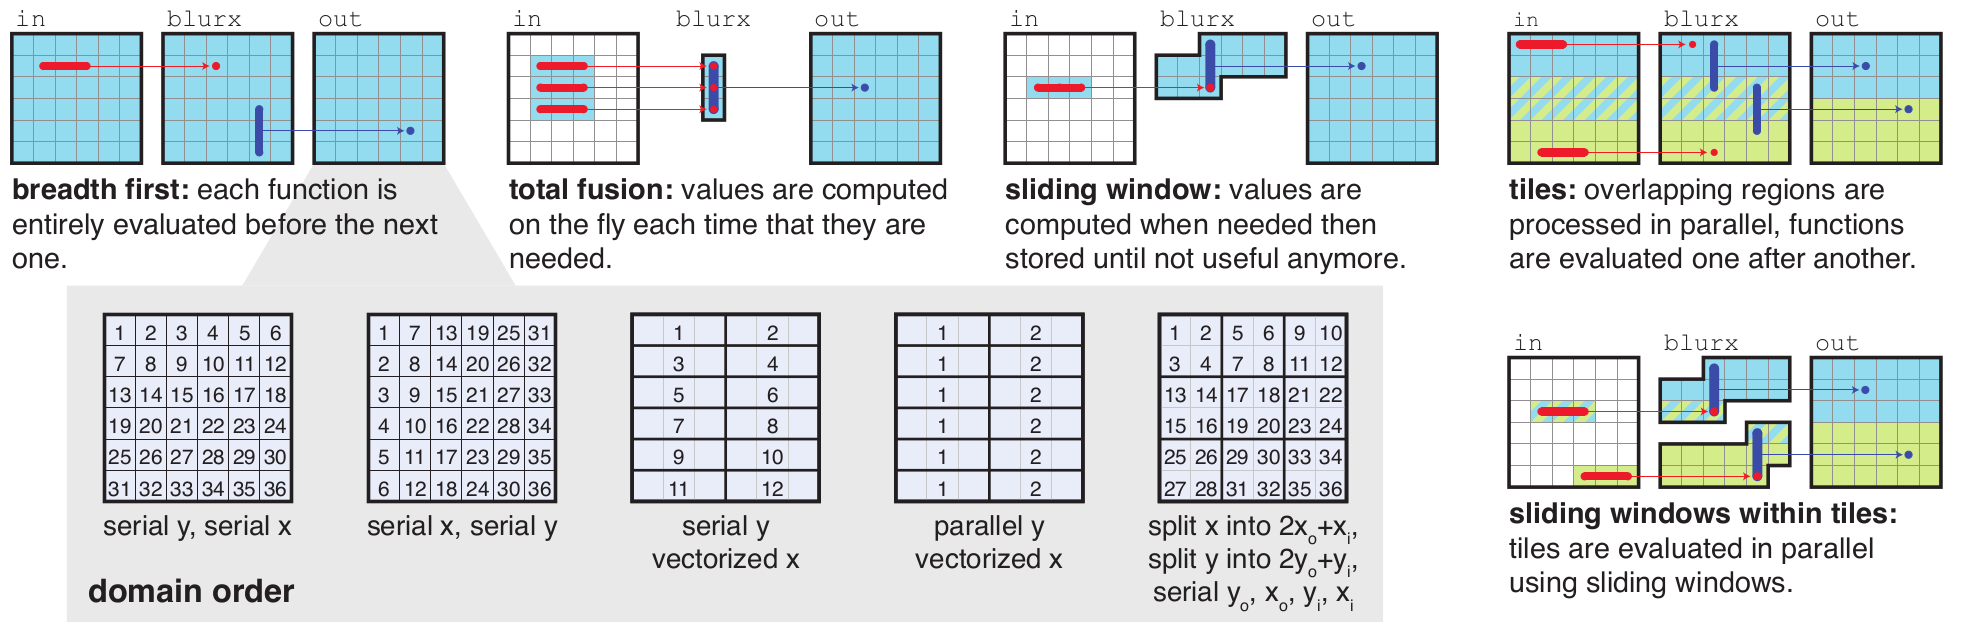
\includegraphics[width=11cm]{simple_pipline.png}
    \caption{box filter的几种可能的Schedule方案}
    \label{fig:schedule-example}
  \end{figure}
  
\end{frame}

\section{DSL-Halide}
\begin{frame}
  \begin{block}{直接优化代码}
    \begin{itemize}
    \item 对程序员有很高的要求.
    \item 费力耗时
    \item 且代码与平台相关性高不易移植.
    \end{itemize}
  \end{block}
  
  \begin{exampleblock}{Using Halide}
    \begin{itemize}
    \item Schedule 和 Algorithm分离
    \item 支持多种平台代码生成(cpu, metal, opengl, cuda ...)
    \end{itemize}
  \end{exampleblock}
\end{frame}

\begin{frame}
  \frametitle{Halide-Example}
  \begin{figure}[H]
    \centering
    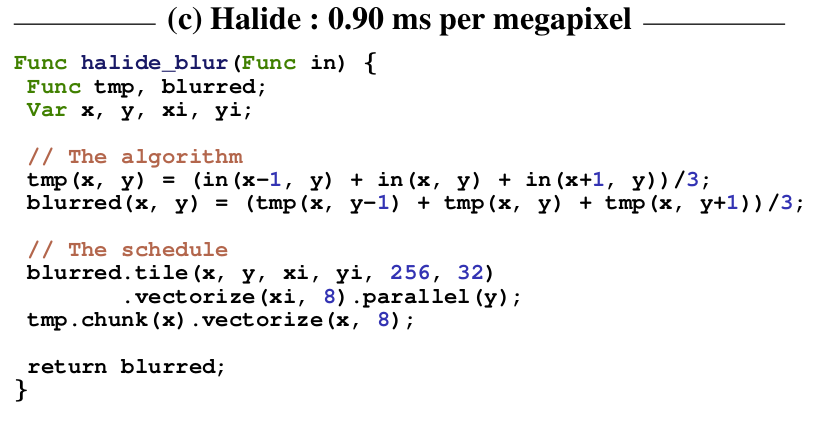
\includegraphics[width=10cm]{halide_box_filter.png}
    \caption{halide box filter代码实现}
    \label{fig:halide-box-filter}
  \end{figure}
\end{frame}

\begin{frame}
  \frametitle{自动调优}
  Schedule独立, 方便了性能调优, 但任然需要耗时费力的尝试.\\

  有没有办法, 自动得到一个好的方案?
\end{frame}

\begin{frame}
  \frametitle{解空间的建模}
  Schedule变化可以总结为两个方面:
  \begin{itemize}
  \item The Domain Order, 定义了每个函数空间的遍历方式
    \begin{itemize}
    \item 顺序/并行
    \item 循环展开以及矢量化
    \item column major/row major
    \item 拆分为多个小片, 按片遍历
    \end{itemize}
  \item The Call Schedule, 定义了函数存储和计算的粒度如:
    \begin{itemize}
    \item breadth-first, 先计算blur-x存储起来, 然后再计算blur
    \item fused, 每次重新计算blur-x
    \item sliding-window
    \end{itemize}
  \end{itemize}
\end{frame}

\begin{frame}
  \frametitle{解空间的搜索}
  变化的空间非常大, 使用遗传算法, 并通过一些先验来搜索. 一些策略:
  \begin{itemize}
  \item 从breadth-first开始进行搜索
  \item 片的长度的选择为2的整数倍
  \item 同一个函数采用相同的策略
  \item ...
  \end{itemize}
\end{frame}

\begin{frame}
  \frametitle{Compiler Pipeline}
  \begin{figure}[H]
    \centering
    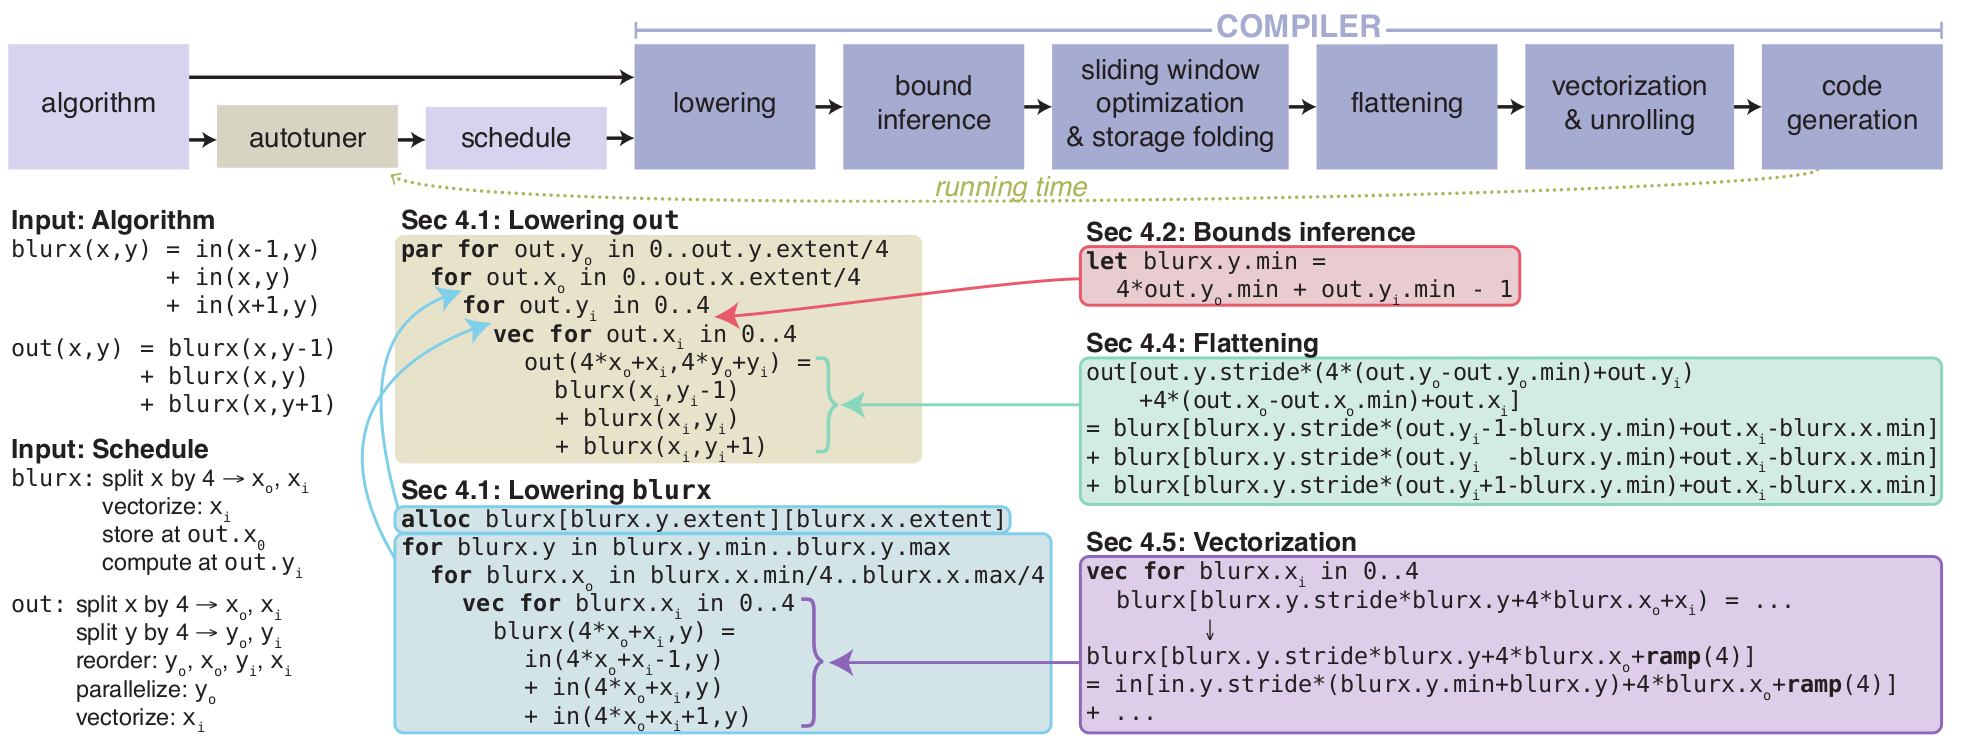
\includegraphics[width=11cm]{compiler_pipeline.png}
    \caption{编译流程}
    \label{fig:compiler-pipeline}
  \end{figure}
\end{frame}

\begin{frame}
  \frametitle{Reference}
  \begin{itemize}
  \item \href{http://people.csail.mit.edu/jrk/halide12}{\textcolor{blue}{Decoupling Algorithms from Schedules\\
    for Easy Optimization of Image Processing Pipelines}}
  \item \href{http://people.csail.mit.edu/jrk/halide-pldi13.pdf}{\textcolor{blue}{Halide: A Language and Compiler for Optimizing Parallelism,\\
    Locality, and Recomputation in Image Processing Pipelines}}
  \end{itemize}
\end{frame}

%% \begin{block}{title of the bloc}
%%   bloc text
%% \end{block}

%% \begin{exampleblock}{title of the bloc}
%%   bloc text
%% \end{exampleblock}

%% \begin{alertblock}{title of the bloc}
%%   bloc text
%% \end{alertblock}

\end{document}
